\begin{figure}[H]
	\begin{center}
	\caption{Pilar de elevador com cargas distintas nos diferentes ramos.}
	\label{figura-pilar-de-elevador-cargas-distintas}
    	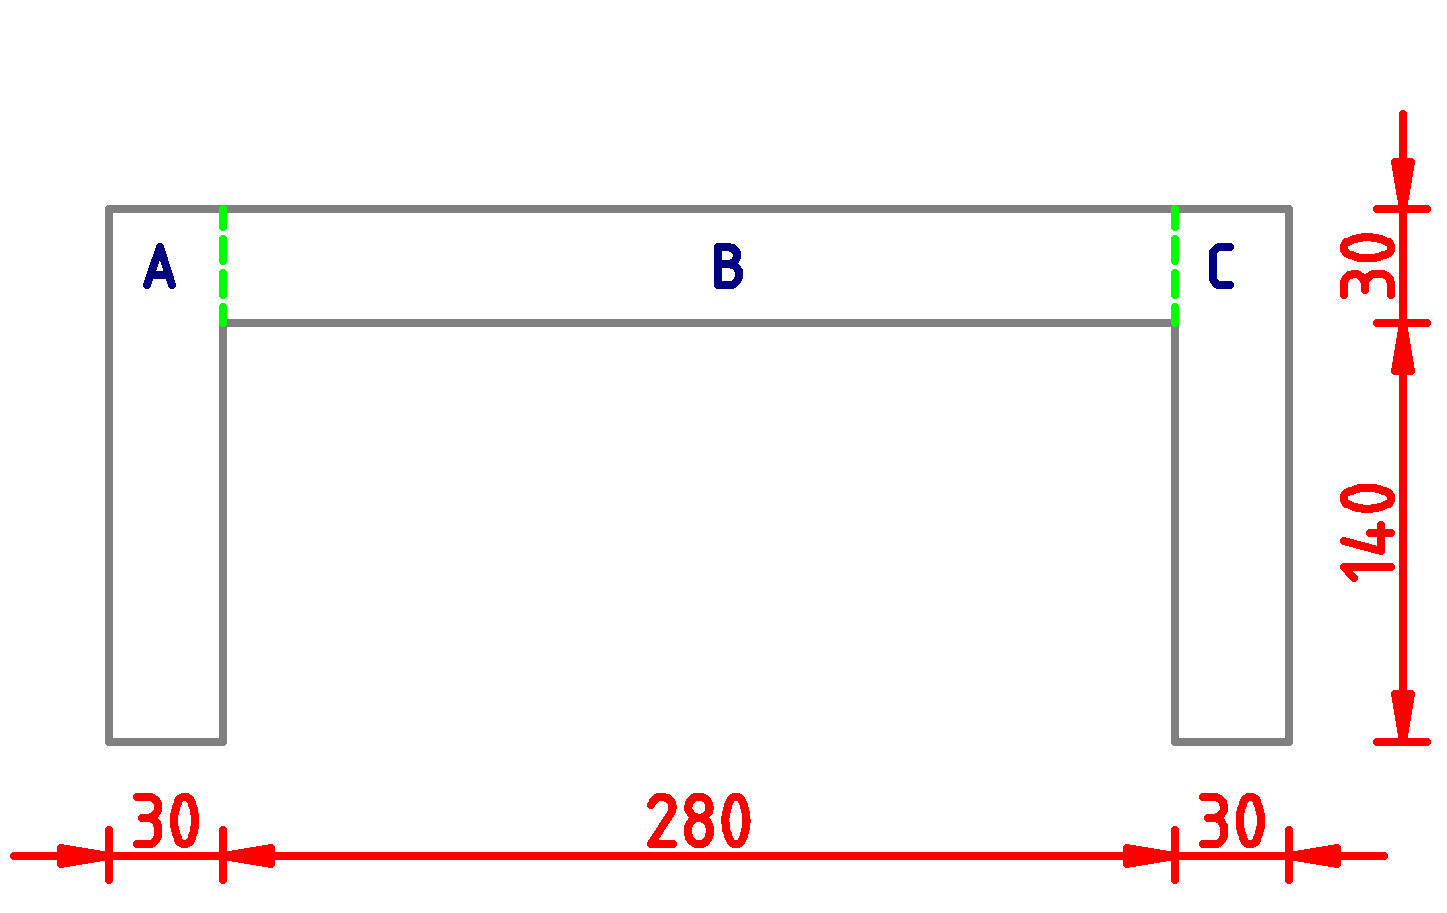
\includegraphics[width=0.4\textwidth]{Fundacoes-rasas-ou-diretas/Imagens/Pilares-com-cargas-distintas-nos-diferentes-ramos.png}
	\end{center}
\end{figure}

Cargas: $A=5000\;kN/m^2$, $B=6000\;kN/m^2$ e $C=7000\;kN/m^2$.

Deve-se montar um pilar retangular fictício onde o seu centro de carga (CC) coincida com o centro de carga do pilar da Figura~\ref{figura-pilar-de-elevador-cargas-distintas}. Encontra-se o ponto de centro de carga baseado numa média ponderada das cargas de cada ramo, como segue:
\begin{equation}
	\label{equacao-xcc}
	x_{CC}=\frac{\displaystyle\sum_{i=1}^n P_i\cdot \overline{x}_i}{\displaystyle\sum_{i=1}^n P_i}
\end{equation}
\begin{equation}
	\label{equacao-ycc}
	y_{CC}=\frac{\displaystyle\sum_{i=1}^n P_i\cdot \overline{y}_i}{\displaystyle\sum_{i=1}^n P_i}
\end{equation}

O primeiro passo é converter as cargas que estão por $m^2$ em cargas pontuais, ou seja, o produto entre a carga por $m^2$ e a área da respectiva peça:
$$\text{A}=5000\;kN/m^2\cdot(0,3\;m\cdot1,7\;m)=2550\;kN$$
$$\text{B}=6000\;kN/m^2\cdot(2,8\;m\cdot0,3\;m)=5040\;kN$$
$$\text{C}=7000\;kN/m^2\cdot(0,3\;m\cdot1,7\;m)=3570\;kN$$

A carga total $P$ é, portanto:
$$P=2550\;kN+5040\;kN+3570\;kN=11160\;kN$$

A coordenada $x_{CC}$ pela Equação~\eqref{equacao-xcc}:
$$x_{CC}=\frac{2550\;kN\cdot0,15\;m+5040\;kN\cdot1,7\;m+3570\;kN\cdot3,25\;m}{11160\;kN}\approx1,84\;m$$

A coordenada $y_{CC}$ pela Equação~\eqref{equacao-ycc}:
$$y_{CC}=\frac{2550\;kN\cdot0,85\;m+5040\;kN\cdot1,55\;m+3570\;kN\cdot0,85\;m}{11160\;kN}\approx1,17\;m$$

Como $x_{CC}=1,84\;m$, essa distância é a maior entre as faces das extremidades nesse eixo até o centro de carga, portanto, o valor de $a_0$ (maior lado do pilar fictício retangular):
$$a_0=2\cdot x_{CC}=2\cdot1,84\;m=3,68\;m$$

Da mesma maneira, como $y_{CC}=1,17\;m$ é a maior distância entre as faces das extremidades nesse eixo até o centro de carga, o valor de $b_0$ (menor lado do pilar fictício retangular):
$$b_0=2\cdot y_{CC}=2\cdot1,17\;m=2,34\;m$$

A área de sapata isolada necessária:
$$A=\frac{P}{\sigma_s}=\frac{11160\;kN}{300\;\frac{kN}{m^2}}\approx37,2\;m^2$$

A área necessária é, também, o produto dos seus lados. Logo, o lado $a$ é:
$$a=\frac{A}{b}=\frac{37,2\;m^2}{b}$$

Pode-se substituir o valor de $a$, $a_0$ e $b_0$ na Equação~\eqref{equacao-equilibrio-balancos}:
$$a-a_0=b-b_0$$
$$\frac{37,2}{b}-3,68=b-2,34$$

Multiplicando ambos os lados por $b$ e igualando a zero:
$$b^2+1,34\cdot b-37,2=0$$

Encontrando as raízes por Bhaskara:
$$x_{1,2}=\frac{-b\pm\sqrt{b^2-4\cdot a \cdot c}}{2\cdot a}=\frac{-1,34\pm\sqrt{1,34^2-4\cdot 1 \cdot (-37,2)}}{2\cdot 1}$$
$$x_1\approx5,46\;m\approx5,5\;m$$
$$x_2\approx-6,805\;m\approx-6,85\;m$$

Portanto, $a=6,85\;m$ e $b=5,5\;m$.